% Print
\documentclass[DIV=15,headinclude]{scrartcl}

%Für Tablets:
%\documentclass{scrartcl}
%\usepackage[margin=5mm,a5paper,includefoot]{geometry}

%Packages, die für die deutsche Sprache erforderlich sind
\usepackage[utf8]{inputenc}
\usepackage[T1]{fontenc}
\usepackage[ngerman]{babel}
\usepackage{csquotes}

% Schönere Schriftart
\usepackage[sfdefault]{roboto}

%Packages für Graphik
\usepackage{graphicx}
\graphicspath{{Abbildungen/}}

%BibLaTex
%\usepackage[backend=biber]{biblatex}
%\addbibresource{../Literatur/Literaturliste.bib} 

%Package, damit Bibtex-URL klappt
\usepackage{hyperref}
\usepackage{url}

%Noch schönere Typographie
%\usepackage{microtype}

%Package für schöne Tabellen mit variabler Breite
\usepackage{tabulary}
\usepackage{booktabs}

% Todo
\usepackage[german]{todonotes}

% Draft
\usepackage{draftwatermark}
\SetWatermarkText{Entwurf}
\SetWatermarkScale{0.5}

%Kasten
\usepackage{framed}

%Fancy Headers
\usepackage[headsepline,footsepline]{scrlayer-scrpage}
\pagestyle{scrheadings}
\ohead{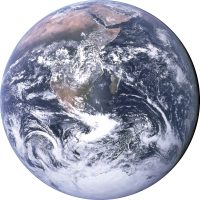
\includegraphics[height=1cm]{bluemarble}}
\chead{\headmark}
\automark{section}
%\ihead{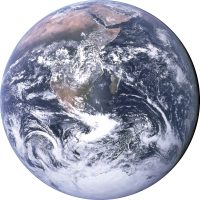
\includegraphics[height=1cm]{bluemarble.jpg}}
\ifoot{\csname @title\endcsname}\cfoot{\pagemark}
\ofoot{\today}

\begin{document}
%%%%% BEGINN TITEL %%%%%
\title{Prüfungsleistungen und Bewertungskriterien}
\subtitle{Entwicklungsmethoden für Nachhaltige Produkte}
\author{Abhishek Gupta \and Ludger Heide}
\maketitle
%%%%% ENDE TITEL %%%%%

\tableofcontents

%%%%% BEGINN INHALT %%%%%

\listoftodos

\section{Über dieses Dokument}

\section{Prüfungsleistungen}

\begin{table}
	\centering
	\caption{Zusammensetzung der Gesamtnote}
	\label{tab:zusammensetzung}
	\begin{tabular}{lrr}
		\toprule
		Name & Typ & Gewichtung \\
		\midrule
		Lernjournal & individuell & 50 \% \\		
		Präsentation & Gruppe & 10 \% \\
		Projektbericht & Gruppe & 40 \% \\	
		\bottomrule
	\end{tabular}
\end{table}

Die Veranstaltung ist als Portfolioprüfung\footnote{Rahmenbedingugen: \href{https://www.tu-berlin.de/asv/menue/gremien/kommissionen_des_as/hinweise_zur_allgstupo/hinweise_zu_portfoliopruefungen/}{\underline{hier}}} konzipiert. Tabelle \ref{tab:zusammensetzung} zeigt die Zusammensetzung der Gesamtnote auf die einzelnen Teilleistungen.

\begin{table}
	\centering
	\caption{Notenschlüssel}
	\label{tab:notenschlüssel}
	\begin{tabular}{lr}
		\toprule
		Punktzahl & Note \\
		\midrule
		$\geq$ 85 & 1,0 \\
		$\geq$ 80 & 1,3 \\
		$\geq$ 75 & 1,7 \\
		$\geq$ 70 & 2,0 \\
		$\geq$ 65 & 2,3 \\
		$\geq$ 60 & 2,7 \\
		$\geq$ 55 & 3,0 \\
		$\geq$ 50 & 3,3 \\
		$\geq$ 45 & 3,7 \\
		$\geq$ 40 & 4,0 \\
		$<$ 40  & 5,0 \\
		\bottomrule
	\end{tabular}
\end{table}

Zur Zuordnung der Portfoliopunkte zu den Noten kommt der "`Notenschlüssel 3"' der Fakultät IV zur Anwendung, wie in Tabelle \ref{tab:notenschlüssel} gezeigt. Dieser Notenschlüssel ist "`großzügiger"' als die üblicherweise an der Fakultät V verwendeten. Wir wollen eine Lehrveranstaltung, in der "`sehr gut"' nicht "`fehlerfrei"' bedeuten muss und wir nicht eine Korrektur für die Punkte machen und eine, in der wir alle Fehler auszählen, die uns zwar aufgefallen sind aber für die wir keine Punkte abziehen können, weil sonst die Note zu schlecht wird. Studierende sollten also damit rechnen, das die Punktzahlen der Teilleistungen schlechter als gewohnt ausfallen, die Noten jedoch nicht.

\subsection{Lernjournal}

\subsubsection{Beschreibung}
\emph{Ziel} des Lernjournals ist es, sich mit den vermittelten Inhalten selbstständig erneut auseinanderzusetzen und sie in einem sorgfältig erstellten Dokument aufzubereiten. Neben der Reproduktion sollen hier auch eigene Einschätzungen und Interpretationen der Inhalte vermerkt werden.

\emph{Formell} werden keine umfangreichen Anforderungen gestellt. Eine "`wissenschaftliche"' Form (z.~B. so wie dieses Dokument) ist genauso akzeptabel wie eine kreativere Auseinandersetzung mit Mindmaps, Zeichnungen und viel buntem Papier. Die Abgabe kann physisch oder elektronisch erfolgen.

Wir erwarten einen \emph{Umfang} von ein bis zwei A4-Seiten (oder dem Äquivalent dazu in anderen Formaten) für jeden Themenblock.

\subsubsection{Bewertungskriterien}

\begin{description}
	\item[Selbstständigkeit] Die Aufgabe sollte jede Studentin selbstständig ohne fremde Hilfe durchführen.
	\item[Äußere Form] Es sollte einfach erkennbar sein, wer Autorin ist und um was es sich handelt.
	\item[Vollständigkeit] Wir erwarten, dass jeder Themenblock bearbeitet wird.
	\item[Inhalt] Wir möchten die Kerninhalte unserer Themenblöcke (oder dass, was die Studierenden als Kerninhalte wahrnehmen) wiedererkennen.
	\item[Struktur] Die Inhalte sollten sinnvoll Anhalt des \emph{Inhalts} strukturiert und kategorisiert sein, nicht bloß so, wie dir Vorlesung ablief.
	\item[Eigene Gedanken] War es für euch neu oder schon bekannt? War es logisch schlüssig oder unerwartet? Glaubt ihr, das die Inhalte des Themenblockes so stimmen, oder kritisiert ihr unsere Meinungen und Fakten?
	\item[Form] Das Lernjournal sollte frei von Rechtschreib-, Grammatik- und Zeichenfehlern und (ungewollten) Stilbrüchen sein.
\end{description}

Die Bepunktung der Bewertungskriterien ist in Abbildung \ref{abb:lernjournal} zu sehen.

\begin{figure}
  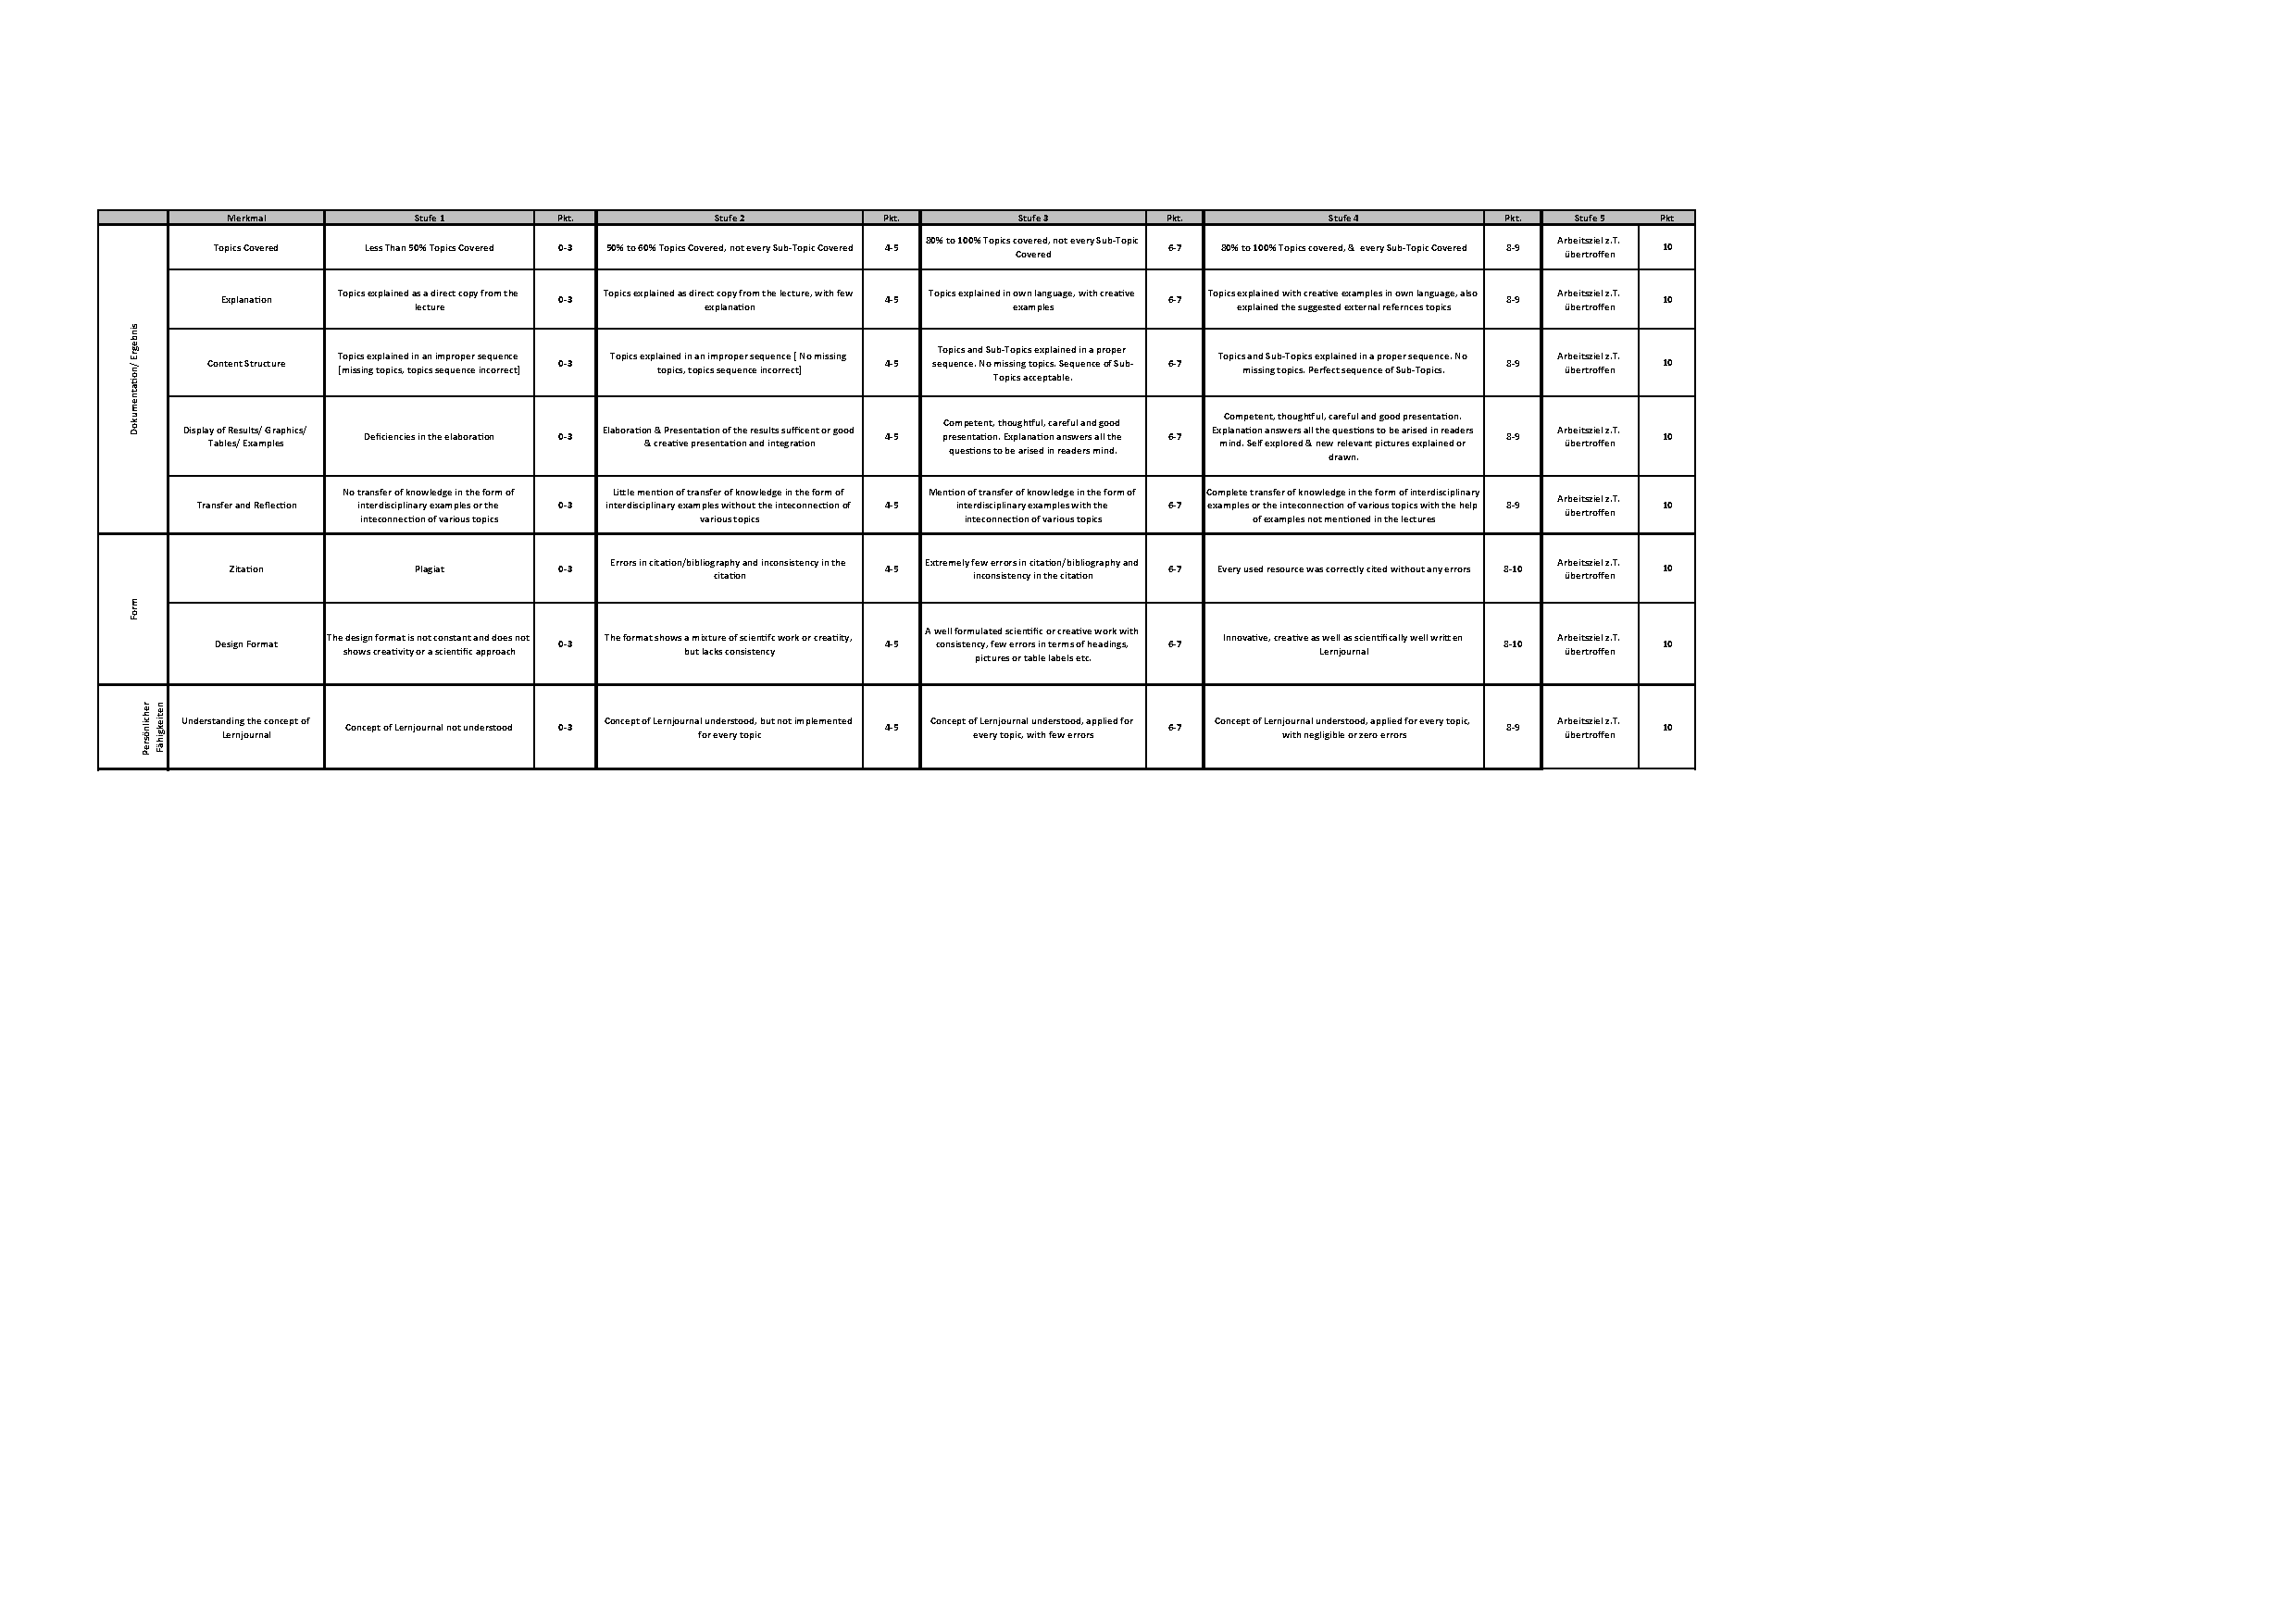
\includegraphics[width=\linewidth]{lernjournal}
  \caption{Bewertungskriterien Lernjournal}s
  \label{abb:lernjournal}
\end{figure}

\subsection{Präsentation}

\subsubsection{Beschreibung}

\emph{Ziel} der Präsentation ist es, eure Ergebnisse zu einer Teilaufgabe des Projektes mit euren Kolleginnen zu teilen und eine Diskussion darüber zu führen. Es soll \emph{nicht} um eine bloße – am schlimmsten noch bei allen Gruppen gleiche – Projektpräsentation gehen, sondern um die Gestaltung einer Mini-Lehreinheit zu einem bestimmten Thema.

\emph{Formell} wird ein Zeitrahmen von 30 Minuten und eine Wissensvermittlung und Diskussion mit allen Teilnehmern gefordert. Voraussichtlich muss die Präsentation online stattfinden. Weitere Anforderungen (Medium, Software, Redeanteile) gibt es nicht.

\subsubsection{Bewertungskriterien}

\todo[inline, caption={Bewertungskriterien Präsentation}]{Bewertungskriterien Präsentation – orientieren an bisherigen Präsentationen am Fachgebiet MPM, aber Interaktivität/Diskussionsgestaltung einbeziehen}

\subsection{Projektbericht}

\subsubsection{Beschreibung}

\todo[inline, caption={Beschreibung Projektbericht}]{Beschreibung des Projektberichts – kongruent mit der Aufgabenstellung, die @Anne Syré macht}

\subsubsection{Bewertungskriterien}

\todo[inline, caption={Bewertungskriterien Projektbericht}]{Bewertungskriterien Projektbericht – orientieren an "`Methodisches Konstruieren"' und "`Electric Vehicle Technologies and Applications"'}

%%%%% ENDE INHALT %%%%%

%Bibliographie
%\printbibliography

\end{document}
